% !TeX root = RJwrapper.tex
\title{New Tools for Performing Financial Analysis Using the ``Tidy''
Split-Apply-Combine Framework}
\author{by Matt Dancho, Davis Vaughan}

\maketitle

\abstract{%
Financial analysis and data science in the R programming language have
followed two separate yet innovative paths resulting in two different
but important systems, ``xts'' and ``tidyverse''. The ``xts'' system has
advantages with the management of financial data, while the
``tidyverse'' has advantages with scaling using the
\emph{split-apply-combine} framework. Because of the separation in
development, the two systems are difficult to use together, which limits
the full potential of financial analysis within R. The
\texttt{tidyquant} packages solves this problem by integrating several
of the best financial analysis packages with the ``tidy'' ecosystem, in
the process unlocking the benefits of the \emph{split-apply-combine}
framework.

Two usage cases are discussed to illustrate the potential. The first
example uses the scaling capabilities to provide an answer for how the
``market'' values risk versus reward. The second example evaluates
methods to scale the performance analysis of multiple portfolios using
combinations of weighted blends. These examples just scratch the surface
of the full potential as technology develops, and future possibilities
are briefly addressed.
}

\section{Status of Financial Analysis Tools in
R}\label{status-of-financial-analysis-tools-in-r}

The R programming language has seen immense growth in both popularity
and tools over the past several years primarily driven by the
open-source nature of the R language and innovation in the field of data
science. The sub-segment of financial analysis in R is no different.
\href{https://timelyportfolio.github.io/rCharts_time_series/history.html}{TimelyPortfolio}
maintains a timeline of the major advances in R time series graphics,
which highlights the inception of several of the most influential R
financial and time series packages. Several packages are worth
describing in more detail as these create much of the current foundation
of R in Finance.

\begin{figure}[htbp]
  \centering
  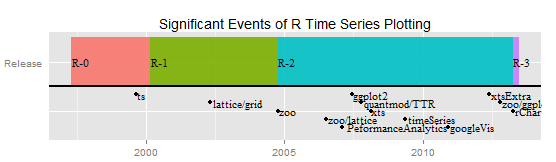
\includegraphics[width=14cm]{img/timeline}
\end{figure}

\subsection{quantmod / TTR}\label{quantmod-ttr}

The \emph{Quantitative Financial Modelling \& Trading Framework for R}
(\texttt{quantmod}) package and the \emph{Technical Trading Rules}
(\texttt{TTR}) package include mechanisms to retrieve, compute, and
visualize financial data using the most popular technical trading rules.

\subsection{xts / zoo}\label{xts-zoo}

The \emph{Extensible Time Series} (\texttt{xts}) package along with the
\texttt{zoo} package include mechanisms for the handling of time series
data. Most importantly, the \texttt{xts} package implemented a
cross-package method for handling the various time series data
structures, in the process solving a major shortcoming by managing
\emph{all major R time series objects}
\footnote{At least the following time series data objects exist in R to solve general and specific needs: `fts`, `its`, `irts`, `timeSeries`, `ti`, `ts`, `mts`, `zoo`, and `xts`. The sheer volume of options results in a complex decision process to determine which to use.}
under one class, \texttt{xts}.

\subsection{PerformanceAnalytics}\label{performanceanalytics}

The \texttt{PerformanceAnalytics} package includes a large collection of
econometric functions for financial performance analysis, many of which
are described in \emph{Practical Portfolio Performance Measurement and
Attribution} by Carl Bacon \citep{Bacon2004} . These functions enable
analysis of individual asset and portfolio (the weighted aggregation of
multiple assets) returns using popular statistical methods for measuring
performance.

\section{New Tools: tidyverse}\label{new-tools-tidyverse}

In parallel with the progression in the R in Finance community,
developers at \emph{RStudio} have been developing useful tools for data
science in R, namely the ``tidyverse''. The ``tidyverse'' or ``tidy''
ecosystem is a collection of packages that fundamentally and
philosophically work together utilizing ``tidy'' data, which is defined
in \emph{Tidy Data} \citep{tidy-data}. Further, the ``tidyverse''
packages and the data analysis workflow are documented in the online
text, \emph{R for Data Science} \citep{R4DS2017}, which is the de facto
manual for data scientists beginning with the R programming language.
The ``tidyverse'' includes several packages worth describing in more
detail.

\begin{figure}[htbp]
  \centering
  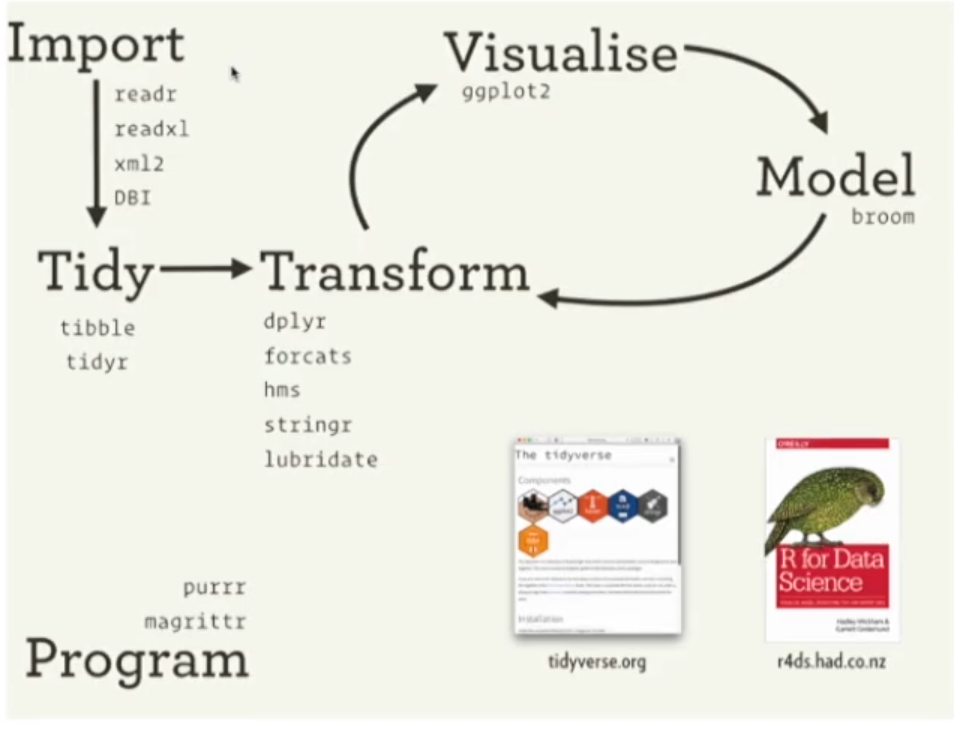
\includegraphics[width=12cm, height=8cm]{img/tidyverse}
\end{figure}

\subsection{dplyr / tidyr}\label{dplyr-tidyr}

The \texttt{dplyr} and \texttt{tidyr} packages provide tools to clean
and manipulate data using the \emph{split-apply-combine} framework
popularized by Hadley Wickham in \emph{The Split-Apply-Combine Strategy
for Data Analysis} \citep{plyr}. The major advances were threefold.
First, the packages simplified and made consistent many of the most
common data manipulation and summarization tasks in R. Second, the
packages enable the \emph{split-apply-combine} framework to work with
grouped data sets. Third, the packages incorporated the use of the pipe
(\texttt{\%\textgreater{}\%}) from the \texttt{magrittr} package,
enabling functional verbs to follow an easy, efficient, and
human-readable workflow.

\subsection{purrr}\label{purrr}

The \texttt{purrr} package provides tools for applying functions to data
frames. Similar to the traditional \texttt{apply} function in base R,
the \texttt{map} function enables ``mapping'' functions row-wise within
a data frame. The major advance is the ability to scale analysis. An
analysis can be performed with ``nested'' data frames allowing users to
apply functions across many independent data sets, a common task in data
science. Further, the resulting data frame is ``tidy'', meaning each
analysis result is kept alongside the data that generated it.

\subsection{tibble}\label{tibble}

The \texttt{tibble} package extends the traditional \texttt{data.frame}
object by providing useful tools for creating and coercing objects to
``tibbles'' or ``tidy'' data frames.

\subsection{ggplot2}\label{ggplot2}

The \texttt{ggplot2} package provides mechanisms for creating complex
visualizations using a layered approach called the ``grammar of
graphics'', which is discussed in \emph{A Layered Grammar of Graphics}
\citep{layered-grammar}. The \texttt{ggplot2} package is the primary
package for creating static graphics in the ``tidy'' ecosystem.

\subsection{lubridate}\label{lubridate}

The \texttt{lubridate} package includes functions to manage date and
date-time objects in R, which is discussed in \emph{Dates and Times Made
Easy with lubridate} \citep{lubridate}. The combination of
\texttt{lubridate} with \texttt{dplyr} enables easy coercion of
character class to date and date-time, filtering and subsetting on
dates, and many more complex tasks that are essential to financial
analysis. Further, combining \texttt{lubridate} with \texttt{ggplot2}
enables graphical visualization using dates and date-times.

\section{Divergent Philosophies, Each with
Advantages}\label{divergent-philosophies-each-with-advantages}

All of the major financial packages work within the ``xts'' system,
which is specifically designed for time series analysis. The system
works very well. The extensible time series, ``xts'', data structure is
much like a numeric matrix, the only major visible difference being row
names consisting of the date or date-time information. The objects can
be subset or transformed to different periodicity very easily. The
disadvantage is that the application is strict to numeric data, but
because of its focus it manages the numeric time-based data extremely
well.

Much of the recent innovation in data analysis has occurred within the
``tidy'' ecosystem. With the entrance of the ``tidyverse'', scaling
analysis using the \emph{split-apply-combine} framework has become easy,
efficient, and core functionality. Further, advances in date and
date-time functionality have enabled management of time series data
within the ``tibble'' data structure. As the data science field grows,
more innovative functionality will continue to be developed within the
``tidy'' ecosystem, much of which will be (and is already) useful to the
field of financial analysis.

The two systems, ``xts'' and the ``tidyverse'', are very different on a
fundamental and philosophical level. Both have advantages that are
needed within the realm of financial analysis, but unfortunately the two
systems do not work well together. The ``xts'' system is strictly
numeric-based, while the ``tidy'' system is strictly data frame-based.
Passing data between systems is difficult if not painful, and without
communication between each the full potential of financial analysis
within R is limited.

To solve this problem, the \texttt{tidyquant} package was developed as a
way to integrate many of the ``xts'' based financial analysis packages
into the ``tidyverse''. The central motivation behind the integration is
to enable the user to gain the benefits of both systems. The
\texttt{tidyquant} package works with ``tidy'' input and output, and as
a result fits seamlessly within the ``tidy'' ecosystem allowing for
analysis to follow the data science workflow discussed in detail in
\emph{R for Data Science} \citep{R4DS2017}. Internally,
\texttt{tidyquant} leverages the ``xts'' system as the engine to perform
financial computations. This enables almost all of the functionality of
\texttt{quantmod}, \texttt{TTR}, \texttt{PerformanceAnalytics},
\texttt{xts} and \texttt{zoo} to be used integrally (without switching
back and forth) within the ``tidy'' ecosystem. The primary benefit of
this integration is the ability to implement the
\emph{split-apply-combine} framework to scale complex analysis.

In the next section, the \emph{split-apply-combine} framework is
discussed using non-financial data, followed by a demonstration of the
\texttt{tidyquant} package to illustrate some of its key benefits within
the realm of financial analysis.

\section{Split-Apply-Combine, The
Concept}\label{split-apply-combine-the-concept}

The \emph{split-apply-combine} framework is described in \emph{The
Split-Apply-Combine Strategy for Data Analysis} \citep{plyr}. To
summarize, the core concept is to split a data set into groups, apply
functions to independent groups, and then recombine the results. The
value in this approach is that the framework enables scaling analyses
from one group to many groups and comparing each group to each other.

A simple example using the \texttt{mtcars} data set illustrates this
framework. The \texttt{mtcars} data set includes the various attributes
for 32 vehicles along with the fuel efficiency (MPG) of each vehicle.

Start with a question: \emph{How does engine size affect fuel
consumption?}

\begin{Schunk}
\begin{Sinput}
# Load the tidyverse and the mtcars data set in R.
library(tidyverse)
data("mtcars")
\end{Sinput}
\end{Schunk}

Next, view the data set. The \texttt{as\_tibble} function is used to
convert to the ``tidy'' data frame structure. The data set consists of
12 columns (features) and 32 rows (observations) related to various
automobiles. Fortunately, the frame of the question narrows the analysis
to two variables: ``mpg'', continuous numeric data describing the fuel
efficiency of each vehicle, and ``cyl'', discrete numeric data
indicating number of engine cylinders for each vehicle. The ``cyl'' data
can be grouped on to keep like observations together.

\begin{Schunk}
\begin{Sinput}
mtcars <- mtcars %>%
    rownames_to_column(var = "model") %>%
    as_tibble()
head(mtcars)
\end{Sinput}
\end{Schunk}

\begin{tabular}{cccccccccccc}
\toprule
model & mpg & cyl & disp & hp & drat & wt & qsec & vs & am & gear & carb\\
\midrule
Mazda RX4 & 21.0 & 6 & 160 & 110 & 3.90 & 2.620 & 16.46 & 0 & 1 & 4 & 4\\
Mazda RX4 Wag & 21.0 & 6 & 160 & 110 & 3.90 & 2.875 & 17.02 & 0 & 1 & 4 & 4\\
Datsun 710 & 22.8 & 4 & 108 & 93 & 3.85 & 2.320 & 18.61 & 1 & 1 & 4 & 1\\
Hornet 4 Drive & 21.4 & 6 & 258 & 110 & 3.08 & 3.215 & 19.44 & 1 & 0 & 3 & 1\\
Hornet Sportabout & 18.7 & 8 & 360 & 175 & 3.15 & 3.440 & 17.02 & 0 & 0 & 3 & 2\\
Valiant & 18.1 & 6 & 225 & 105 & 2.76 & 3.460 & 20.22 & 1 & 0 & 3 & 1\\
\bottomrule
\end{tabular}

\hspace{20 mm}

Many solutions exist to compare fuel consumption and engine size. For
simplicity, the mean and standard deviation are used to characterize the
relationship between number of cylinders and miles per gallon.
Implementing \emph{split-apply-combine} is as easy as grouping by a
categorical variable and summarizing by the target measure. In this
case, the categorical variable is the ``cyl'' variable.

\begin{Schunk}
\begin{Sinput}
mtcars %>%
    mutate(cyl = factor(cyl)) %>%
    group_by(cyl) %>%
    summarize(mpg.mean = mean(mpg),
              mpg.sd = sd(mpg))
\end{Sinput}
\end{Schunk}

\begin{tabular}{ccc}
\toprule
cyl & mpg.mean & mpg.sd\\
\midrule
4 & 26.66364 & 4.509828\\
6 & 19.74286 & 1.453567\\
8 & 15.10000 & 2.560048\\
\bottomrule
\end{tabular}

\hspace{20 mm}

From the results, the vehicles, when grouped by ``cyl'', appear to have
an inverse relationship between number of cylinders and miles per
gallon. We can also visualize this relationship using \texttt{ggplot2}.

\begin{Schunk}
\begin{Sinput}
mtcars %>%
    mutate(cyl = factor(cyl)) %>%
    ggplot(aes(x = cyl, y = mpg, fill = cyl)) +
    geom_boxplot() +
    labs(title = "Summarizing Relationships using Split-Apply-Combine",
         subtitle = "Inverse Relationship between Engine Size and Fuel Efficiency",
         x = "Engine Size (# of Cylinders)",
         y = "Fuel Efficiency (MPG)")
\end{Sinput}


\begin{center}\includegraphics{RInFinanceRticles_files/figure-latex/unnamed-chunk-7-1} \end{center}

\end{Schunk}

The \emph{split-apply-combine} framework is used to solve a wide range
of complex problems. In the next section, examples are presented to
illustrate the power of unlocking the framework combined with data
science workflow tools within financial analysis applications.

\section{Split-Apply-Combine, Applications in
Finance}\label{split-apply-combine-applications-in-finance}

The financial analysis packages are difficult or impossible to use
within the ``tidy'' ecosystem. A new tool is needed, \texttt{tidyquant}.
The \texttt{tidyquant} package has one major advance: it integrates the
``xts'' based financial packages with the ``tidyverse'' to enable the
data science workflow and ``tidy'' ecosystem functionality to be applied
to financial analysis. The innovation is relatively minor on a
conceptual level, but the net effect is significant in that the tools
within the ``tidy'' ecosystem are now unlocked for financial analysis.
The following examples illustrate the new capability.

\subsection{Example 1: Evaluating Risk vs
Reward}\label{example-1-evaluating-risk-vs-reward}

Financial analysis is almost always a trade off between risk and reward.
Reward is measured by growth of an investment. Risk is typically
associated with volatility. Often when beginning an analysis, one wishes
to understand the components of a market basket of stocks on the basis
of this risk-reward trade off in order to screen investments.

Start with a question: \emph{How does the market value risk versus
reward?}

This question is answerable by comparing the risk and reward
characteristics for a basket of stocks viewed as a reasonable proxy for
the ``market''. The observations within the market are stocks. Stocks
also have observations or historical prices, which can be obtained over
time and can be used to evaluate various statistical qualities that
relate to risk versus reward. The reward is the return performance
(i.e.~returns), which is the positive or negative percentage change
between observations. When accumulated across a frequency such as daily,
the large set of returns has statistical properties that can be
measured. To simplify the question, the average and standard deviation
of the returns can be used as a general proxy of risk versus reward.
When pooled together, the stocks can thus be compared to expose general
performance trends within the market.
\footnote{Using the mean and standard deviation of stock returns has roots in Brownian motion and is known as the Stochastic Process, which is often used in Monte Carlo simulation to predict the range of future returns within a confidence interval based on the properties of the past returns. }

To start, load \texttt{tidyquant}, which loads all of the packages
needed to evaluate risk versus reward.

\begin{Schunk}
\begin{Sinput}
# Loads tidyquant, tidyverse, lubridate, quantmod, TTR, xts, zoo, PerformanceAnalytics
library(tidyquant)
\end{Sinput}
\end{Schunk}

Next, collect some financial data. The question implies that a large
sample of stock data is needed to evaluate how performance and risk is
valued within the ``market''. The S\&P 500 index is a good place to
start. \texttt{tidyquant} includes a function, \texttt{tq\_index}, which
returns the stock symbols and company names for every stock within an
index.

\begin{Schunk}
\begin{Sinput}
sp500 <- tq_index("SP500")
head(sp500)
dim(sp500)
\end{Sinput}
\end{Schunk}

\begin{tabular}{cc}
\toprule
symbol & company\\
\midrule
MMM & 3M\\
ABT & ABBOTT LABORATORIES\\
ABBV & ABBVIE INC\\
ACN & ACCENTURE\\
ATVI & ACTIVISION BLIZZARD\\
AYI & ACUITY BRANDS\\
\bottomrule
\end{tabular}

{[}1{]} 502 2

\hspace{20 mm}

Next, we need the historical stock prices for each stock within the S\&P
500 index. The stock prices are easy to retrieve at scale using the
function, \texttt{tq\_get}, with the ``get'' option,
\texttt{get\ =\ "stock.prices"}. \texttt{tq\_get} is a wrapper for
\texttt{quantmod::getSymbols}, which enables passing the underlying
function parameters \texttt{from} and \texttt{to}. The input to
\texttt{tq\_get} is \texttt{data}, which can be a single stock symbol, a
vector of stock symbols, or a data frame with stock symbols in the first
column. The latter is passed to \texttt{tq\_get} using the pipe
(\texttt{\%\textgreater{}\%}). The function may take a few minutes to
run because it is downloading the past ten years of daily open, high,
low, close, volume, and adjusted stock prices for the entire S\&P 500
index into one ``tidy'' data frame. Reviewing the results indicates that
the prices were retrieved in entirety. The resulting ``tibble'' has
1,205,845 rows and 502 unique symbols.

\begin{Schunk}
\begin{Sinput}
sp500_stock_prices <- sp500 %>%
    tq_get(get  = "stock.prices", 
           from = "2007-01-01", 
           to   = "2017-01-01")
head(sp500_stock_prices)
dim(sp500_stock_prices)
\end{Sinput}
\end{Schunk}

\begin{tabular}{ccccccccc}
\toprule
symbol & company & date & open & high & low & close & volume & adjusted\\
\midrule
MMM & 3M & 2007-01-03 & 77.53 & 78.85 & 77.38 & 78.26 & 3781500 & 60.31064\\
MMM & 3M & 2007-01-04 & 78.40 & 78.41 & 77.45 & 77.95 & 2968400 & 60.07174\\
MMM & 3M & 2007-01-05 & 77.89 & 77.90 & 77.01 & 77.42 & 2765200 & 59.66330\\
MMM & 3M & 2007-01-08 & 77.42 & 78.04 & 76.97 & 77.59 & 2434500 & 59.79431\\
MMM & 3M & 2007-01-09 & 78.00 & 78.23 & 77.44 & 77.68 & 1896800 & 59.86367\\
MMM & 3M & 2007-01-10 & 77.31 & 77.96 & 77.04 & 77.85 & 1787500 & 59.99468\\
\bottomrule
\end{tabular}

{[}1{]} 1205845 9

\hspace{20 mm}

Next, the \emph{split-apply-combine} framework is used to group the
prices by stock symbol and to calculate the logarithmic daily returns.
The transform is applied using \texttt{tq\_transform}, which is used in
situations where periodicity changes (or can change). The
\texttt{quantmod} OHLC (open, high, low, close) notation is used to
collect the adjusted prices (\texttt{ohlc\_fun\ =\ Ad}) and send these
prices to the \texttt{periodReturn} function
(\texttt{transform\_fun\ =\ periodReturn}). The additional arguments
\texttt{period\ =\ "daily"} and \texttt{type\ =\ "log"} are passed to
the transformation function, \texttt{periodReturn}. The daily log
returns (DLR) for each of the 502 groups of stock symbols is generated
below.

\begin{Schunk}
\begin{Sinput}
sp500_returns <- sp500_stock_prices %>%
    group_by(symbol) %>%
    tq_transform(ohlc_fun = Ad, transform_fun = periodReturn, 
                 period = "daily", type = "log", col_rename = "dlr")
head(sp500_returns)
\end{Sinput}
\end{Schunk}

\begin{tabular}{ccc}
\toprule
symbol & date & dlr\\
\midrule
MMM & 2007-01-03 & 0.0000000\\
MMM & 2007-01-04 & -0.0039691\\
MMM & 2007-01-05 & -0.0068224\\
MMM & 2007-01-08 & 0.0021934\\
MMM & 2007-01-09 & 0.0011593\\
MMM & 2007-01-10 & 0.0021860\\
\bottomrule
\end{tabular}

\hspace{20 mm}

Next, the mean and standard deviation of the daily log returns are used
to evaluate and compare the stocks. The easiest way is to use
\texttt{tq\_performance}, which applies the
\texttt{PerformanceAnalytics} performance functions to ``tidy'' data
frames of asset or portfolio returns. The \texttt{table.Stats} function
returns the arithmetic mean and standard deviation along with a number
of other useful statistics that characterize the returns.

\begin{Schunk}
\begin{Sinput}
sp500_stats <- sp500_returns %>%
    tq_performance(Ra = dlr, performance_fun = table.Stats, ci = 0.95, digits = 6) 
sp500_stats %>%
    select(1:5) %>%
    head()
\end{Sinput}
\end{Schunk}

\begin{tabular}{ccccc}
\toprule
symbol & ArithmeticMean & GeometricMean & Kurtosis & LCLMean(0.95)\\
\midrule
MMM & 0.000431 & 0.000331 & 5.806040 & -0.000120\\
ABT & 0.000302 & 0.000215 & 6.294066 & -0.000211\\
ABBV & 0.000714 & 0.000565 & 3.868658 & -0.000350\\
ACN & 0.000543 & 0.000404 & 8.532566 & -0.000108\\
ATVI & 0.000604 & 0.000359 & 10.735599 & -0.000263\\
AYI & 0.000701 & 0.000420 & 6.011008 & -0.000225\\
\bottomrule
\end{tabular}

\hspace{20 mm}

Finally, we have the data needed to visualize risk versus reward. A plot
of the mean daily log returns (MDLR) versus the standard deviation of
daily log returns (SDDLR) shows the relationship. Note that observations
(stocks) with fewer than five years of trading days (5 years x 252 trade
days per year) are removed from the visualization to yield a long-run
perspective.

\begin{Schunk}
\begin{Sinput}
sp500_stats %>%
    filter(Observations >= 252 * 5) %>%
    ggplot(aes(x = Stdev, y = ArithmeticMean)) +
    geom_point(alpha = 0.5, col = "steelblue") +
    geom_smooth(method = "lm") +
    labs(title = "Evaluating Risk Vs Reward for Stocks in the SP500",
         subtitle = "An inverse trend between volatility (SDDLR) and returns (MDLR)",
         x = "Standard Deviation of Daily Log Returns (SDDLR)",
         y = "Arithmetic Mean of Daily Log Returns (MDLR)") +
    theme_tq()
\end{Sinput}


\begin{center}\includegraphics{RInFinanceRticles_files/figure-latex/unnamed-chunk-17-1} \end{center}

\end{Schunk}

By comparing an entire basket of stocks, reasonable trading strategies
can be developed. For example, creating a portfolio that minimizes
volatility may result in higher performance over the long run. This is
easily seen in the trend line indicating an inverse trend between
volatility (SDDLR) and returns (MDLR). Further, once trading strategies
are developed, screening is easily implemented by filtering the data
set.

\begin{Schunk}
\begin{Sinput}
sp500_stats %>%
    filter(Observations >= 252 * 5,
           Stdev <= 0.02,
           ArithmeticMean >= 0.0005) %>%
    arrange(desc(ArithmeticMean)) %>%
    select(1:5) %>%
    head()
\end{Sinput}
\end{Schunk}

\begin{tabular}{ccccc}
\toprule
symbol & ArithmeticMean & GeometricMean & Kurtosis & LCLMean(0.95)\\
\midrule
TDG & 0.00116 & 0.00097 & 7.96994 & 0.00039\\
FBHS & 0.00111 & 0.00094 & 2.58643 & 0.00011\\
DLPH & 0.00094 & 0.00079 & 4.21629 & 0.00000\\
ROST & 0.00090 & 0.00073 & 5.15896 & 0.00019\\
ORLY & 0.00086 & 0.00070 & 10.20942 & 0.00016\\
AGN & 0.00082 & 0.00067 & 6.06114 & 0.00013\\
\bottomrule
\end{tabular}

\hspace{20 mm}

\subsection{Example 2: Evaluating Performance of Multiple Portfolio
Blends}\label{example-2-evaluating-performance-of-multiple-portfolio-blends}

Portfolio aggregation is a useful technique to reduce risk while
maintaining acceptable returns. In this example, the goal is to evaluate
a few blended portfolios of ``FANG'' stocks (``FB'', ``AMZN'', ``NFLX'',
and ``GOOG'').
\footnote{The acronymn, "FANG", was popularized by Jim Cramer of the popular CNBC show, Mad Money. http://www.investopedia.com/terms/f/fang-stocks-fb-amzn.asp.}
However, more important is the conceptual idea that the number of
weighted portfolio blends and the number of underlying assets can easily
be increased to scale the analysis. As the example progresses, consider
how this could be applied to an entire index of assets and hundreds of
weighted blends.

Throughout the past half decade, the FANG stocks have experienced a
unique combination of high returns and high volatility, making the FANG
stocks a good example to use in a blended portfolio that reduces
downside risk but yields high returns.

Start with a question: \emph{What portfolio blends reduce downside risk
while maximizing return?}

Several portfolio blends will be evaluated to see the historical effect
on returns since 2013:
\footnote{2013 was the first full year of trading data for FB. Portfolio aggregation prior to 2013 cannot be analyzed with FB.}

\begin{itemize}
\tightlist
\item
  Portfolio 1: 50\% FB, 25\% AMZN, 25\% NFLX, 0\% GOOG
\item
  Portfolio 2: 0\% FB, 50\% AMZN, 25\% NFLX, 25\% GOOG
\item
  Portfolio 3: 25\% FB, 0\% AMZN, 50\% NFLX, 25\% GOOG
\item
  Portfolio 4: 25\% FB, 25\% AMZN, 0\% NFLX, 50\% GOOG
\end{itemize}

First, collect the data for the ``FANG'' stocks.

\begin{Schunk}
\begin{Sinput}
FANG <- c("FB", "AMZN", "GOOG", "NFLX") %>%
    tq_get(get = "stock.prices")
slice(FANG, 1:6)
\end{Sinput}
\end{Schunk}

\begin{tabular}{cccccccc}
\toprule
symbol & date & open & high & low & close & volume & adjusted\\
\midrule
FB & 2012-05-18 & 42.05 & 45.00 & 38.00 & 38.23 & 573576400 & 38.23\\
FB & 2012-05-21 & 36.53 & 36.66 & 33.00 & 34.03 & 168192700 & 34.03\\
FB & 2012-05-22 & 32.61 & 33.59 & 30.94 & 31.00 & 101786600 & 31.00\\
FB & 2012-05-23 & 31.37 & 32.50 & 31.36 & 32.00 & 73600000 & 32.00\\
FB & 2012-05-24 & 32.95 & 33.21 & 31.77 & 33.03 & 50237200 & 33.03\\
FB & 2012-05-25 & 32.90 & 32.95 & 31.11 & 31.91 & 37149800 & 31.91\\
\bottomrule
\end{tabular}

\hspace{20 mm}

Next, transform to monthly returns using the \emph{split-apply-combine}
framework. Use \texttt{group\_by} to group on the ``symbol'' column, and
\texttt{tq\_transform} to transform the adjusted prices to monthly
arithmetic returns. Note that ``FB'' was only actively traded for a full
year beginning in 2013, so it makes sense to compare the investments
since then.

\begin{Schunk}
\begin{Sinput}
FANG_returns <- FANG %>%
    filter(date >= ymd("2013-01-01"),
           date <  ymd("2017-01-01")) %>%
    group_by(symbol) %>%
    tq_transform(ohlc_fun = Ad,
                 transform_fun = periodReturn,
                 period = "monthly",
                 col_rename = "returns")
slice(FANG_returns, 1:2)
\end{Sinput}
\end{Schunk}

\begin{tabular}{ccc}
\toprule
symbol & date & returns\\
\midrule
AMZN & 2013-01-31 & 0.0318293\\
AMZN & 2013-02-28 & -0.0046328\\
FB & 2013-01-31 & 0.1064286\\
FB & 2013-02-28 & -0.1204003\\
GOOG & 2013-01-31 & 0.0448531\\
\addlinespace
GOOG & 2013-02-28 & 0.0602232\\
NFLX & 2013-01-31 & 0.7958918\\
NFLX & 2013-02-28 & 0.1382232\\
\bottomrule
\end{tabular}

\hspace{20 mm}

\subsubsection{Individual Asset
Performance}\label{individual-asset-performance}

Before the portfolios are generated and evaluated, it makes sense to
visualize and assess the performance of the individual asset returns.
The first visualization uses a wealth index, which takes an initial
investment as an input and returns a visualization showing how the
investment would have grown over the specified time period. From the
visualization, NFLX was the best performer, but it also experienced some
significant drops along the way.

\begin{Schunk}
\begin{Sinput}
init_investment <- 10000
FANG_wealth <- FANG_returns %>%
    mutate(wealth.index = init_investment * cumprod(1 + returns))

FANG_wealth %>%
    ggplot(aes(x = date, y = wealth.index, color = symbol)) +
    geom_line(size = 2) +
    geom_smooth(method = "loess") +
    labs(title = "Individual Stocks: Comparing the Growth of 10K",
         x = "", y = "Investment Value") +
    theme_tq() +
    scale_color_tq() +
    scale_y_continuous(labels = scales::dollar)
\end{Sinput}


\begin{center}\includegraphics{RInFinanceRticles_files/figure-latex/unnamed-chunk-24-1} \end{center}

\end{Schunk}

Because of the volatility, the risk should be evaluated as well. One
popular method to measure risk is using value at risk (VaR). VaR
measures the worst expected loss over a given time interval under normal
market conditions, at a given confidence level \citep{Bacon2004}.
Implementing VaR can be done using \texttt{tq\_performance} with the
\texttt{PerformanceAnalytics} function, \texttt{VaR}, to estimate risk
measures across the FANG stocks. While NFLX and AMZN returns are
stellar, the VaR risk estimate is also double that of FB and GOOG.

\begin{Schunk}
\begin{Sinput}
VaR_FANG <- FANG_returns %>%
    tq_performance(Ra = returns, Rb = NULL, performance_fun = VaR, p = 0.95) %>%
    rename(VaR.monthly = VaR) 
VaR_FANG
\end{Sinput}
\end{Schunk}

\begin{tabular}{cc}
\toprule
symbol & VaR.monthly\\
\midrule
FB & -0.0564358\\
AMZN & -0.0968790\\
GOOG & -0.0566269\\
NFLX & -0.0977580\\
\bottomrule
\end{tabular}

\hspace{20 mm}

From the results, a portfolio consisting entirely of one of the assets
could yield great results, but it's not for the risk averse. A better
method might be to use a weighted aggregation within a portfolio.

\subsubsection{Portfolio Performance}\label{portfolio-performance}

Weighted portfolio aggregation involves three steps:

\begin{enumerate}
\def\labelenumi{\arabic{enumi}.}
\tightlist
\item
  Make a portfolio by repeating the stock returns table \emph{n} times
\item
  Create a weights table to map weights by asset and portfolio
\item
  Aggregate the portfolios using \texttt{tq\_portfolio}, a wrapper for
  \texttt{PerformanceAnalytics::Return.portfolio}
\end{enumerate}

\paragraph{Step 1: Make a portfolio by repeating the stock
returns}\label{step-1-make-a-portfolio-by-repeating-the-stock-returns}

Use \texttt{tq\_repeat\_df} to repeat \texttt{n\ =\ 4} times. This
function extends the data frame row-wise, adding an index column named
``portfolio'' and grouping by ``portfolio''. We now have four portfolio
groups that will be evaluated.

\begin{Schunk}
\begin{Sinput}
FANG_returns_mult <- FANG_returns %>%
    tq_repeat_df(n = 4)
slice(FANG_returns_mult, 1:2)
\end{Sinput}
\end{Schunk}

\begin{tabular}{cccc}
\toprule
portfolio & symbol & date & returns\\
\midrule
1 & FB & 2013-01-31 & 0.1064286\\
1 & FB & 2013-02-28 & -0.1204003\\
2 & FB & 2013-01-31 & 0.1064286\\
2 & FB & 2013-02-28 & -0.1204003\\
3 & FB & 2013-01-31 & 0.1064286\\
\addlinespace
3 & FB & 2013-02-28 & -0.1204003\\
4 & FB & 2013-01-31 & 0.1064286\\
4 & FB & 2013-02-28 & -0.1204003\\
\bottomrule
\end{tabular}

\hspace{20 mm}

\paragraph{Step 2: Create a Weights
Table}\label{step-2-create-a-weights-table}

Construct a weights table using the portfolio blending parameters, which
will be used to map to the portfolios in the next step. The format of
the weights table is critical. The table must have three columns,
``portfolio'', ``stocks'', and ``weights''. Make sure to group by the
portfolio column.

\begin{itemize}
\tightlist
\item
  Portfolio 1: 50\% FB, 25\% AMZN, 25\% NFLX, 0\% GOOG
\item
  Portfolio 2: 0\% FB, 50\% AMZN, 25\% NFLX, 25\% GOOG
\item
  Portfolio 3: 25\% FB, 0\% AMZN, 50\% NFLX, 25\% GOOG
\item
  Portfolio 4: 25\% FB, 25\% AMZN, 0\% NFLX, 50\% GOOG
\end{itemize}

\begin{Schunk}
\begin{Sinput}
weights <- c(0.50, 0.25, 0.25, 0.00,
             0.00, 0.50, 0.25, 0.25,
             0.25, 0.00, 0.50, 0.25, 
             0.25, 0.25, 0.00, 0.50)
weights_table <- tibble(stocks = c("FB", "AMZN", "NFLX", "GOOG")) %>%
    tq_repeat_df(n = 4) %>%
    bind_cols(tibble(weights)) %>%
    group_by(portfolio)
weights_table
\end{Sinput}
\end{Schunk}

\begin{tabular}{ccc}
\toprule
portfolio & stocks & weights\\
\midrule
1 & FB & 0.50\\
1 & AMZN & 0.25\\
1 & NFLX & 0.25\\
1 & GOOG & 0.00\\
2 & FB & 0.00\\
\addlinespace
2 & AMZN & 0.50\\
2 & NFLX & 0.25\\
2 & GOOG & 0.25\\
3 & FB & 0.25\\
3 & AMZN & 0.00\\
\addlinespace
3 & NFLX & 0.50\\
3 & GOOG & 0.25\\
4 & FB & 0.25\\
4 & AMZN & 0.25\\
4 & NFLX & 0.00\\
4 & GOOG & 0.50\\
\bottomrule
\end{tabular}

\hspace{20 mm}

\paragraph{Step 3: Aggregate the Portfolios with
tq\_portfolio}\label{step-3-aggregate-the-portfolios-with-tq_portfolio}

Aggregate the portfolios using \texttt{tq\_portfolio}, a wrapper for
\texttt{PerformanceAnalytics::Return.portfolio}. The
\texttt{Return.portfolio} has additional arguments to create a wealth
index, which is the compounded returns. Setting
\texttt{wealth.index\ =\ TRUE} and multiplying the result by the initial
investment value of \$10,000 returns a wealth index. The performance of
the various blended portfolios is visualized using \texttt{ggplot2} with
the aesthetic argument, \texttt{color\ =\ factor(portfolio)}.

\begin{Schunk}
\begin{Sinput}
# Aggregate portfolio with tq_portfolio. Pass wealth.index = TRUE
init_investment <- 10000
FANG_portfolio_wealth <- FANG_returns_mult %>%
    tq_portfolio(assets_col = symbol, returns_col = returns,
                 weights = weights_table, wealth.index = TRUE,
                 col_rename = "wealth.index") %>%
    mutate(wealth.index = wealth.index * init_investment)

FANG_portfolio_wealth  %>%
    ggplot(aes(x = date, y = wealth.index, color = factor(portfolio))) +
    geom_line(size = 2) +
    geom_smooth(method = "loess") +
    labs(title = "Portfolios: Comparing the Growth of 10K",
         subtitle = "Quickly visualize blended portfolio performance",
         x = "", y = "Investment Value",
         color = "Portfolio Number: ") +
    theme_tq() +
    scale_color_tq() +
    scale_y_continuous(labels = scales::dollar)
\end{Sinput}


\begin{center}\includegraphics{RInFinanceRticles_files/figure-latex/unnamed-chunk-31-1} \end{center}

\end{Schunk}

Finally, the risk is assessed in the same manner as the individual
assets. The portfolio aggregation is performed without the
\texttt{wealth.index} option, which aggregates uncompounded returns. The
returns are ``piped'' to the \texttt{tq\_performance} function, which
returns the VaR.

\begin{Schunk}
\begin{Sinput}
VaR_portfolio <- FANG_returns_mult %>%
    tq_portfolio(assets_col = symbol, returns_col = returns,
                 weights = weights_table, col_rename = "returns") %>%
    tq_performance(Ra = returns, Rb = NULL, performance_fun = VaR) %>%
    rename(VaR.monthly = VaR)
VaR_portfolio
\end{Sinput}
\end{Schunk}

\begin{tabular}{cc}
\toprule
portfolio & VaR.monthly\\
\midrule
1 & -0.0853386\\
2 & -0.1055108\\
3 & -0.1077418\\
4 & -0.0526966\\
\bottomrule
\end{tabular}

\hspace{20 mm}

The two tables below summarize the results of the individual and
portfolio analyses, respectively. The Portfolio 1 blend is an attractive
combination of growth with lower risk: over 5.1X return with over a 1\%
decrease in the VaR of both NFLX and AMZN. To further optimize, one
could run algorithms to identify the ``best'' minimum variance
portfolio.

\hspace{20 mm}

\begin{tabular}{ccc}
\toprule
symbol & value.end & VaR.monthly\\
\midrule
AMZN & 29142.67 & -0.0968790\\
FB & 41089.29 & -0.0564358\\
GOOG & 21364.41 & -0.0566269\\
NFLX & 94185.41 & -0.0977580\\
\bottomrule
\end{tabular}

\hspace{20 mm}

\begin{tabular}{ccc}
\toprule
portfolio & value.end & VaR.monthly\\
\midrule
1 & 51376.66 & -0.0853386\\
2 & 43458.79 & -0.1055108\\
3 & 62706.13 & -0.1077418\\
4 & 28240.19 & -0.0526966\\
\bottomrule
\end{tabular}

\hspace{20 mm}

\section{Future Possibilities}\label{future-possibilities}

The \emph{split-apply-combine} framework presents an opportunity for
progress in the realm of financial analysis due to the scale at which
analysis can now be performed. Portfolio analysis is especially
interesting because as the number of components and the number of
portfolio blend variations increase, the number of potential portfolio
combinations become infinite. Yet, with the scaling capabilities within
the ``tidy'' ecosystem, the vast array of possibilities becomes limited
only by the data storage and processing capabilities of the computers on
which the computations are performed. With advances in cloud technology,
parallel processing, and optimization algorithms, the tools are
available to scale analyses to terabytes worth of financial data in real
time. The work is not complete, but, as innovation continues, financial
analysis will benefit from both speed and scale.

\bibliography{RJreferences}

\address{%
Matt Dancho\\
Business Science\\
\\
}
\href{mailto:mdancho@business-science.io}{\nolinkurl{mdancho@business-science.io}}

\address{%
Davis Vaughan\\
Business Science\\
\\
}
\href{mailto:dvaughan@business-science.io}{\nolinkurl{dvaughan@business-science.io}}


